-\setcounter{section}{1} % This causes the next section to be Appendix B


\section*{Examples II: Kinetics, Constitutive Laws, and Viscoelasticity I}
\label{PS2}
\textcolor{red}{(Rev note: v3)}


This set of example problems is due on October 3, 2025. 
As before, I request that you type up your responses in \LaTeX~ rather than write them out by hand. 

\medskip
\subsection*{2--1. \textbf{Balance of mass} [4 pts].} 
A large piece of polydimethylsiloxane (PDMS) of uniform density $\rho(\bm{x},t)$ has a central spherical bubble of time-evolving radius $R(t)$, initial radius $R_0$, and wall velocity of $\dot{R}$. 
The hole is subject to a uniform surface traction in the $\bm{e}^{(r)} \equiv \bm{e}_{\bm{r}}$ direction from an axisymmetric pressure, and maintains spherical symmetry over time. 

\medskip
The position of a point in the material can be written as $\bm{x} = r(R,t) \bm{e}_{\bm{r}}$ with reference position $\bm{X} = r_0(R_0)$, while the velocity of that point can be written as $\bm{v}(r,t) = v_r \bm{e}_{\bm{r}}$.

\medskip
Using the conservation of mass equation, show that the material must satisfy
%\begin{equation}
%\rho_{,t} + (\rho v_i)_{,i} = 0,
%\end{equation}
\begin{equation*}
\rho_{,t}+ \rho_{,r} v_r + \frac{\rho}{r} (\textcolor{red}{2}v_r + r v_{r,r}) = 0,
\end{equation*}
and hence, show that an assumption of incompressibility for PDMS results in 
\begin{equation*}
v_r(r,t) = \frac{R^2 \dot{R}}{r^2}.
\end{equation*}

\bigskip

\textit{Solution.}\\

The balance of mass for a material is written as 

\begin{equation*}
    \frac{\partial\rho}{\partial t} + \mathbf{\nabla}_\mathbf{x} \cdot(\rho\mathbf{v}) = 0 \\
\end{equation*}

Carrying out the derivatives (equation used from Bower Appendix D) and using the fact that $\rho$ and $\mathbf{v}$ are both only functions of times and $r$ (due to axissymmetric nature of the pressure). 


\begin{align*}
    0 &= \rho_{,t} + (\nabla_\mathbf{x}\rho) \cdot \mathbf{v} + \rho(\nabla_{\mathbf{x}}\cdot\mathbf{v}) \\
    &= \rho_{,t} + \left[\frac{\partial\rho}{\partial r}v_r +\frac{1}{r}\frac{\partial\rho}{\partial \theta}v_\theta+\frac{1}{r\sin(\theta)}\frac{\partial\rho}{\partial \phi}\right] + \rho\left[\frac{\partial v_r}{\partial R} + 2\frac{v_r}{R}+\frac{1}{R}\frac{\partial v_\theta}{\partial \theta} + \frac{1}{R\sin(\theta)}\frac{\partial v_\phi}{\partial \phi} + cot(\theta)\frac{v_\theta}{R}\right] \\
    &= \rho_{,t} + \rho_{,r}v_r + \rho\left[v_{r,r}+2\frac{v_r}{r}\right] \\
    &= \rho_{,t} + \rho_{,r}v_r + \frac{\rho}{r}[2v_r + rv_{r,r}] \qed
\end{align*}

To prove the second equation I will begin with the volume balance of two spherical shells. One in the reference configuration between the bubble wall $R_0$ and some larger radius $r_0$ further in the material. Due to incompressibility assumptions, we know that in the deformed configuration, the volume must be the same between the deformed version of the same shell with radii $R(t)$ and $r(t)$, respectively. One extending from the bubble wall between $R_0$ and $R$. The other extends from some arbitrary radius $r_0$ within the material to a larger radius $r$

\begin{align*}
    \frac{4\pi}{3}(r(t)^3-R(t)^3) &= \frac{4\pi}{3}(r_0^3 -R_0^3) \\
     \frac{4\pi}{3}(r(t)^3-r_0^3) &= \frac{4\pi}{3}(R(t)^3 -R_0^3) \\
     r(t)^3-r_0^3 &= R(t)^3 -R_0^3 \\
     r(t) &= (R(t)^3 -R_0^3 + r_0^3)^{1/3} \\
     \frac{dr(t)}{dt} &= \frac{1}{3}(R(t)^3-R_0^3+r_0^3)^{1/3}3R(t)^2\frac{dR(t)}{dt} \\
     &= \frac{1}{3}(r^3)^{-2/3} 3R(t)^2\frac{dR(t)}{dt} \\
     &= r^{-2} R(t)^2\frac{dR(t)}{dt} \\
     v_r(r,t) &= \frac{R(t)^2\dot R(t)}{r^2} \qed \\
\end{align*}

\medskip
\subsection*{2--2. \textbf{Balance of momenta} [4 pts].} A spherical hydrogel body $\mathcal{B}$ with a linear density gradient is currently submerged in water as depicted in the figure. 
The sphere has coordinates $\bm{x}$ in a region $\Omega$ with position-dependent density $\rho(\bm{x})$. 

\begin{figure}[H]
\vspace{-2em}
\centering
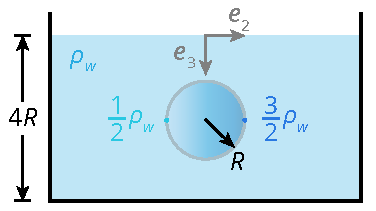
\includegraphics[width=3in]{instr-figures/PS2-Q1.pdf}
\caption{\small{Hydrogel sphere with a linear density gradient submerged in water. The water has a density $\rho_w$, while the sphere has a density at its leftmost point of $\rho_w/2$ and at its rightmost point of $3\rho_w/2$.}}
\end{figure}

\vspace{-1em}
The surface traction $\bm{t}(\bm{x},\hat{\bm{n}})$ acting on $\mathcal{B}$ is given by 
\begin{equation*}
\bm{t}(\bm{x},\hat{\bm{n}}) = -\rho_w g x_3 \hat{\bm{n}},
\end{equation*}
where $\hat{\bm{n}}$ is the outer unit normal to the surface $\partial \Omega_t$ and $\rho_w$ is the (constant) density of water and $g$ is the acceleration due to gravity. 

\medskip
(a) Determine the net force and moment acting on $\mathcal{B}$ via volume integrals.

\medskip
(b) Under what \textit{two} conditions is $\mathcal{B}$ in static equilibrium

\bigskip

\textit{Solution.}\\

\textbf{a.)} There are two forces acting on the bubble. One due to gravitational body force, $F_b$, and the buoyancy due to the traction on the surface, $F_t$. 

\begin{align*}
    F_t &= \int_{\partial \mathcal{B}} \mathbf{t}(\mathbf{x},\hat n)dA_\mathbf{x} \\
    &= \int_{\partial \mathcal{B}}-\rho_wgx_3\mathbf{\hat n}dA_\mathbf{x} \\
    &= -g\int_{\partial \mathcal{B}}\rho_wx_3\mathbf{\hat n}dA_\mathbf{x} \\
    &= -g\rho_w\int_\mathcal{B} \mathbf{\nabla}_\mathbf{x} \cdot \mathbf{\sigma}(x_3)dV_\mathbf{x} \\
    &= -g\rho_w\int_\mathcal{B} \mathbf{\nabla}_\mathbf{x} \cdot x_3 \mathbf{I} dV_\mathbf{x} \\
    &= -g\rho_w\int_\mathcal{B} \frac{\partial(x_3)}{\partial x_3} dV_\mathbf{x} \mathbf{\hat e}^{(3)}\\
    &= -g\rho_w \int_\mathcal{B}dV_\mathbf{x} \mathbf{\hat e}^{(3)}\\
    &= -g\rho_w \frac{4\pi}{3}R^3 \mathbf{\hat e}^{(3)}\\
    F_b &= \int_\mathcal{B}\rho(\mathbf{x}) g dV \mathbf{\hat e}^{(3)} \\
    &= g \int_\mathcal{B}\left(\rho_w + \frac{\rho_w x_2}{2R}\right) dV \mathbf{\hat e}^{(3)}\\
    &= g\rho_w\frac{4\pi}{3}R^3\mathbf{\hat e}^{(3)} + \frac{\rho_w g}{2R}\int_\mathcal{B}x_2dV_\mathbf{x} \mathbf{\hat e}^{(3)} \\
\end{align*}
\begin{align*}
    \Sigma F &= F_t + F_b \\
    &= \frac{\rho_w g}{2R}\int_\mathcal{B}x_2dV_\mathbf{x} \mathbf{\hat e}^{(3)} \\
    &= \frac{\rho_wg}{2R}\int_0^{2\pi} \int_0^\pi \int_0^R \rho\sin(\theta)\sin(\phi) \rho^2\sin(\phi)d\rho d\phi d\theta \mathbf{\hat e}^{(3)}\\
    &= \frac{\rho_wg}{2R}\int_0^{2\pi} \int_0^\pi \int_0^R \rho^3\sin(\theta)\sin^2(\phi)d\rho d\phi d\theta \mathbf{\hat e}^{(3)}\\ 
    &= \frac{\rho_wg}{2R}\int_0^{2\pi} \int_0^\pi \left(\frac{R^4}{4}\right)\sin(\theta)\sin^2(\phi)d\phi d\theta \mathbf{\hat e}^{(3)}\\ 
    &= \frac{\rho_wgR^3}{8}\int_0^{2\pi} \int_0^\pi \sin(\theta)\sin^2(\phi)d\phi d\theta \mathbf{\hat e}^{(3)}\\ 
    &= \frac{\rho_wgR^3}{8}\int_0^{2\pi} \sin(\theta)\left(\frac{\pi}{2}-\frac{1}{4}\sin(2\pi) - \frac{0}{2} + \frac{1}{4}\sin(0)\right) d\theta \mathbf{\hat e}^{(3)}\\ 
    &= \frac{\rho_wgR^3}{8}\int_0^{2\pi} \sin(\theta)\left(\frac{\pi}{2}\right) d\theta \mathbf{\hat e}^{(3)}\\
     &= \frac{\pi \rho_wgR^3}{16}\int_0^{2\pi} \sin(\theta) d\theta \mathbf{\hat e}^{(3)}\\ 
     &= \frac{\pi \rho_wgR^3}{16}(-cos(2\pi) + cos(0)) \mathbf{\hat e}^{(3)}\\
     &= \frac{\pi \rho_wgR^3}{16}(-1 + 1) \mathbf{\hat e}^{(3)}\\
      &= \mathbf{0} \\
\end{align*}

There is no net force in the sphere because it is neutrally buoyant due to it's average density being equal to water. It's centroid of mass is not centered on it's center of geometry so there will be a net moment. 

Now I will move on to calculating the net moment:

\begin{align*}
    \mathbf{M}_t &= \int_{\partial\mathcal{B}}\mathbf{x}\times\mathbf{t}dA_{\mathbf{x}} \\ 
    &= \int_{\partial\mathcal{B}}\mathbf{x}\times\mathbf{\hat n} \cdot \boldsymbol{\sigma} dA_\mathbf{x} \\
    &= \int_{\partial\mathcal{B}} x_i\mathbf{e}^{(i)}\times\sigma_{mj}\hat n_mdA_\mathbf{x} \\&=\int_{\partial\mathcal{B}}\epsilon_{ijk}x_i\sigma_{mj}\hat n_m dA_\mathbf{x}\mathbf{e}^{(k)} \\
    &= \int_{\mathcal{B}} \epsilon_{ijk}\frac{\partial}{\partial x_m}(x_i \sigma_{mj}) dV_\mathbf{x}\mathbf{e}^{(k)} \\
    &= \int_{\mathcal{B}} \epsilon_{ijk}\frac{\partial}{\partial x_m}(-\rho_w g x_3 \delta_{mj} x_i) dV_\mathbf{x}\mathbf{e}^{(k)} \\
    &= -\rho_w g \epsilon_{ijk} \int_\mathcal{B}\frac{\partial}{\partial x_j}(x_i x_3)\mathbf{e}^{(k)}dV_\mathbf{x} \\
    &= -\rho_w g \epsilon_{ijk} \int_\mathcal{B}(\delta_{ij}x_3 + x_i\delta_{3j})\mathbf{e}^{(k)}dV_\mathbf{x} \\
    &= -\rho_w g \int_\mathcal{B}(\epsilon_{iik}x_3 + \epsilon_{i3k}x_i)\mathbf{e}^{(k)}dV_\mathbf{x} \\
    &= -\rho_w g \int_\mathcal{B} \epsilon_{i3k}x_i\mathbf{e}^{(k)}dV_\mathbf{x} \\
    &= -\rho_w g \int_\mathcal{B} (-x_1 \mathbf{e}^{(2)} + x_2 \mathbf{e}^{(1)}) dV_\mathbf{x} \\
    &= \mathbf{0} \text{ (from symmetry)}
\end{align*}

Now I will calculate the moment due to the body force. This term we expect to have a non-zero moment due to our density distribution. 

\begin{align*}
    \mathbf{M}_b &= \int_\mathcal{B} \mathbf{x}\times g \rho(\mathbf{x}) \mathbf{e}^{(3)} dV_\mathbf{x} \\
    &= g\int_\mathcal{B} \rho(\mathbf{x})x_i\epsilon_{ij3j}\mathbf{e}^{(j)} \\
    &= g\int_\mathcal{B} \rho(\mathbf{x})(x_2\mathbf{e}^{(1)}-x_1\mathbf{e}^{(2)})dV_\mathbf{x} \\
    &= g\int_\mathcal{B} \left(\rho_w+\frac{\rho_wx_2}{2R}\right)(x_2\mathbf{e}^{(1)}-x_1\mathbf{e}^{(2)})dV_\mathbf{x} \\
\end{align*}

Both terms that just multiply $\rho_w$ will be equal to zero similar to the calculations for $\mathbf{M}_t$. The same symmetry arguements can be used on the $x_1x_2$ term. That leaves one non-trivial integral. 

\begin{align*}
    \mathbf{M}_b &= \frac{g\rho_w}{2R} \mathbf{e}^{(1)} \int_\mathcal{B}x_2^2 dV_\mathbf{x} \\
    &= \frac{g\rho_w}{2R} \mathbf{e}^{(1)} \int_0^{2\pi}\int_0^\pi\int_0^R (\rho\sin(\theta)\sin(\phi))^2\rho^2\sin(\theta)d\rho d\theta d\phi \\
    &= \frac{g\rho_w}{2R} \mathbf{e}^{(1)} \int_0^{2\pi}\int_0^\pi\int_0^R \rho^4\sin^3(\theta)\sin(\phi)d\rho d\theta d\phi \\
    &= \frac{g\rho_w}{2R} \mathbf{e}^{(1)}\left(\frac{R^5}{5}-0\right)\left(\frac{4}{3}\right)(\pi) \\
    &= \frac{2\pi g\rho_wR^4}{15} \mathbf{e}^{(1)} \\
    \mathbf{M} &= \mathbf{M}_b + \mathbf{M}_t \\
    \mathbf{M} &= \frac{2\pi g\rho_wR^4}{15} \mathbf{e}^{(1)} \\
\end{align*}

\textbf{b.)} The hydrogel is at equilibrium if the sum of it's forces and moments are both 0. For force this means that the buoyancy force must be equal to it's weight. The integrals above define the condition for the moment for an arbitrary density distrubtion. 

% \begin{align*}
%     F_b &= \int_\mathcal{B}\rho g dV \mathbf{\hat e}^{(3)} \\
%     &= g \int_\mathcal{B}\left(\rho_w + \frac{x_2}{2R}\right) dV \\
%     &= \frac{g}{2R}
% \end{align*}

\bigskip
\subsection*{2--3. \textbf{Viscoelastic data} [4 pts].} 
Stress relaxation \textcolor{red}{(Ask yourself: does it actually matter whether it's stress relaxation or creep compliance?)} isochrones for a compliant viscoelastic material are shown in the figure below.  

\begin{figure}[H]
\vspace{-1em}
\centering
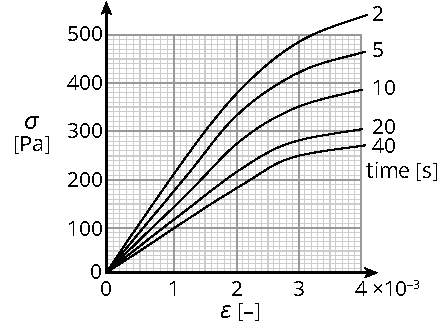
\includegraphics[scale = 1.5]{instr-figures/PS2-Q3.pdf}
\caption{\small{Stress (Pa) vs. strain ($-$) for a soft viscoelastic material.}}
\end{figure}

\vspace{-1em}
(a) Are these isochrones from a material which we can describe with linear viscoelasticity? If not, why not, and if so, under what approximate regimes would this assumption be valid? 

\medskip
(b) Estimate the creep relaxation function $J_c$ for stress values of 100 and 250 \textcolor{red}{Pa}. Isochrones are shown at times of 2, 5, 10, 20, and 40 seconds.   

\bigskip

\textit{Solution.}\\

\textbf{a.)} The material can be described as linear viscoelastic at strains less than or equal to approximately $2\times10^{-3}$ or stresses less than or equal to approximately 240 Pa. In this range the isochrones are each linear which confirms $J_c$ is only a function of $t$. Outside of these regime, all of the curves become nonlinear which shows that $J_c$ also has dependence on $\sigma$ and $t$. By definition, it is no longer in the LVE regime. Please note that in reality the strain/stress box I described is just a rough estimate of the region, a curved line would need to be used to identify the exact region. Also, the material is only LVE for that region for within the ranges of times 2 to 40. Much shorter or longer times may not be LVE in the regime I stated.

\textbf{b.)} In a MATLAB script (pdf attached in submission) I found a best power law script for $\varepsilon_{XXXPa}(t)/\sigma_0 = J_{c,XXXPa}(t)$ for both 100 Pa and 250 Pa. I used this fit because when plotted in loglog the data looked very linear suggesting that it was a reasonable choice of model. My predicted equations were

\begin{align*}
J_{c,100Pa}(t) = 3.4 \cdot 10^{-6} \, t^{0.29} \,[\text{Pa}^{-1}] \\
J_{c,250Pa}(t) = 3.7 \cdot 10^{-6} \, t^{0.31} \,[\text{Pa}^{-1}] \\
\end{align*}

\bigskip
\subsection*{2--4. \textbf{Impulsive stresses} [4 pts].}

(a) Say that instead of a step load, we apply $\sigma(t) = A \delta(t)$ to an unknown linear viscoelastic material. 
Determine the strain history $\epsilon(t)$, first as a general function of the creep relaxation function $J_c(t)$, and then for a Kelvin-Voigt solid. 

(b) Now, consider a rapid load followed by a rapid reverse load by applying a doublet function of stress, i.e. $\sigma(t) = B \psi(t)$. 
What is the strain function $\epsilon(t)$ in terms of $J_c(t)$ and for a Kelvin-Voigt material now? 

\bigskip

\textit{Solution.}\\

\textbf{a.)} 

\begin{align*}
    \varepsilon(t) &= \int_0^t J_c(t-\tau)\frac{d\sigma(\tau)}{d\tau}d\tau \\
    &=  \int_0^t J_c(t-\tau)\frac{d(A\delta(\tau))}{d\tau}d\tau \\
    &=  A\int_0^t J_c(t-\tau)\psi(\tau) d\tau \\
    &= -A\left. \frac{dJc(t-\tau)}{d\tau} \right|_{\tau=0} \\
    \varepsilon_{KV}(t)&= -A\left. \frac{d(\frac{1}{E}(1-\exp(-E(t-\tau)/\eta))}{d\tau} \right|_{\tau=0} \\
    &= -\frac{A}{E} \left.\left( -\frac{E}{\eta}\exp(-E(t-\tau)\eta) \right)\right|_{\tau=0} \\
    &= \frac{A}{\eta}\left.\exp(-E(t-\tau)/\eta) \right|_{\tau=0} \\
    &= \frac{A}{\eta}\exp(-Et/\eta)
\end{align*}

\textbf{b.)} 

\begin{align*}
    \varepsilon(t) &= \int_0^t J_c(t-\tau)\frac{d\sigma(\tau)}{d\tau}d\tau \\
    \varepsilon_{KV}(t) &=  \int_0^t J_c(t-\tau)\frac{d(B\psi(\tau))}{d\tau}d\tau \\
    &= B (-1)^2\left.\frac{d^2J_c(t-\tau)}{d\tau^2}\right|_{\tau=0} \\
    &= B \left.\frac{d^2J_c(t-\tau)}{d\tau^2}\right|_{\tau=0} \\
    &= B \left.\frac{d^2(\frac{1}{E}(1-\exp(-E(t-\tau)/\eta)}{d\tau^2}\right|_{\tau=0} \\
    &= \frac{B}{E} \left.\frac{d^2(1-\exp(-E(t-\tau)/\eta))}{d\tau^2}\right|_{\tau=0} \\
    &= \left. \frac{B}{E} \frac{d(-\frac{E}{\eta} \exp(-E(t-\tau)/\eta)}{d\tau}\right|_{\tau=0}\\
    &= \left. \frac{B}{E} \left(-\frac{E^2}{\eta^2}\exp\left(\frac{-E(t-\tau)}{\eta}\right)\right) \right|_{\tau=0} \\
    &= -\frac{BE}{\eta^2} \exp\left(\frac{-Et}{\eta}\right) \\
\end{align*}


\bigskip
\subsection*{2--5. \textbf{Two-element models} [8 pts].}

Dynamic mechanical analysis (DMA) is a common technique for characterizing viscoelasticity. 
DMA conventionally involves application of a sinusoidal displacement to the top surface of a sample at a controllable temperature. 
Often, the user puts the sample into initial compression, and follows with the sinusoidal profile. 
A cylindrical sample of height $h$ and diameter $d$ is placed between two plates.
The DMA then quickly puts the sample into compression by moving its top plate downward by a displacement $d$, and then oscillates sinusoidally between positions $0$ and $2d$ at a frequency $\omega$.

\medskip
(a) Using the constitutive law for a Kelvin-Voigt material, determine the stress $\sigma(t)$ exerted by the platens to cause the applied strain. 

\medskip
(b) The resulting stress lags behind the strain by an phase $\delta$, as in $\sin(\omega t + \delta)$. 
Commonly this is reported as the ``tangent loss'', or $\tan\delta$, for a material. 
What is the value of $\tan\delta$ for this particular Kelvin-Voigt model?

\medskip
(c) Say instead of prescribing the strain $\epsilon(t)$, we instead prescribed the stress, $\sigma(t) = - \sigma_0 - \sigma_0 \sin(\omega t)$. 
Determine the strain $\epsilon(t)$ for this prescribed stress.

\medskip
(d) Prove that the tangent loss function $\tan\delta$ is identical between the two loading methods.

\bigskip

\textit{Solution.}\\

\textbf{a.)} For a 1D Kelvin-Voigt material we know that:

\begin{equation*}
\sigma(t) = \eta \dot\varepsilon(t) + E\varepsilon(t)
\end{equation*}

The time-dependent strain and strain-rate can be calculated based on the description in the problem description as such: 

\begin{align*}
    \varepsilon(t) &= \frac{d\sin(\omega t)}{h}\\
    \dot\varepsilon &= \frac{d}{h}\frac{\partial(\cos(\omega t))}{\partial t}\\
    &= \frac{d\omega}{h}\cos(\omega t)
\end{align*}

Substituting back into the first equation yields: 

\begin{align*}
    \sigma(t) &= \frac{\eta d\omega}{h} \cos{(\omega t)} + \frac{Ed}{h} \sin{(\omega t)} \\
    &= \frac{d}{h}(\eta \omega \cos{(\omega t)} + E\sin{(\omega t)})
\end{align*}

\textbf{b.)} For the desired phase shifted sine wave we can write in general that

\begin{align*}
    \sin{(\omega t + \delta)} &= \cos{(\delta)}\sin{(\omega t)} + \sin{(\delta)}\cos{(\omega t)} \\
    &= m\sin{(\omega t)} + n\cos{(\omega t)}
\end{align*}

where $m$ and $n$ are constants. Recognize that taking the ratio of these constant terms appended to $\sin{(\omega t)}$ and $\cos{(\omega t)}$ yields:

\begin{align*}
    \frac{n}{m} &= \frac{\sin{(\delta)}}{\cos{(\delta)}} \\
    &= \tan{(\delta)}
\end{align*}

Drawing these constants from the result from part $\bf{a}$ yields

\begin{align*}
    \tan{(\delta)} &= \frac{\eta d w /h}{Ed/h}\\
    &= \frac{\eta w}{E}
\end{align*}

\textbf{c.)} Starting from the constitutive law for a 1D Kelvin-Voigt material

\begin{align*}
    \dot\varepsilon(t) + \frac{E}{\eta}\varepsilon(t) &= \frac{1}{\eta}\sigma(t) \\
    \exp{\left(\frac{Et}{\eta}\right)}\dot\varepsilon(t) + \exp{\left(\frac{Et}{\eta}\right)}\varepsilon(t) &= \frac{1}{\eta}\exp{\left(\frac{Et}{\eta}\right)}\sigma(t) \\
    \frac{d}{dt}\left(\varepsilon(t)\exp{\left(\frac{Et}{\eta}\right)}\right) &= \frac{1}{\eta}\exp{\left(\frac{Et}{\eta}\right)}\sigma(t) \\
\end{align*}

Next I integrate both sides from $0$ to time $t$ so that we can isolate $\varepsilon(t)$ keeping in mind that $\varepsilon(0)$ is equal to $0$.

\begin{align*}
    \varepsilon(t)\exp{\left(\frac{Et}{\eta}\right)} &= \frac{-\sigma_0}{\eta}\int_0^t\exp{\left(\frac{E\tau}{\eta}\right)(1+\sin{(\omega \tau))}}d\tau \\
    &= \frac{-\sigma_0}{\eta} \left[ \int_0^t \exp{\left(\frac{E\tau}{\eta}\right)}d\tau + \int_0^t\exp{\left(\frac{E\tau}{\eta}\right)}\sin{(\omega \tau)}d\tau\right] \\
    &= \frac{-\sigma_0}{\eta} \left[ \frac{\eta}{E}\exp{\left(\frac{Et}{\eta}\right)} - \frac{\eta}{E} + \int_0^t\exp{\left(\frac{E\tau}{\eta}\right)}\sin{(\omega \tau)}d\tau\right]
\end{align*}

The latter integral is more difficult to solve. Let $a$ equal $-E/\eta$. Taking the Laplace transform of the integral and using partial fractions to simplify yields

\begin{align*}
    \mathcal{L}\left[\int_0^t\exp{\left(\frac{E\tau}{\eta}\right)}\sin{(\omega \tau)}d\tau\right](s) &= \mathcal{L}\left[\int_0^t\exp{\left(-a\tau\right)}\sin{(\omega \tau)}d\tau\right](s)\\
    &= \frac{1}{s}\frac{\omega}{(s+a)^2+\omega^2} \\
    &= \frac{\omega}{s(a^2+\omega^2)} - \frac{\omega(s+a)}{(a^2+\omega^2)[(s+a)^2+\omega^2]} - \frac{\omega a
    }{(a^2+\omega^2)[(s+a)^2+\omega^2]} \\
    &= \frac{\omega}{(a^2+\omega^2)}\frac{1}{s} - \frac{\omega}{(a^2+\omega^2)}\frac{(s+a)}{[(s+a)^2+\omega^2]} - \frac{a}{(a^2+\omega^2)}\frac{\omega
    }{[(s+a)^2+\omega^2]} \\
\end{align*}

Using the inverse Laplace transform to solve for the integral result we obtain

\begin{align*}
    \mathcal{L}^{-1}\left[\frac{\omega}{(a^2+\omega^2)}\frac{1}{s} - \frac{\omega}{(a^2+\omega^2)}\frac{(s+a)}{[(s+a)^2+\omega^2]} - \frac{a}{(a^2+\omega^2)}\frac{\omega
    }{[(s+a)^2+\omega^2]} \right](s) = \\\frac{\omega}{(a^2+\omega^2)} - \frac{\omega}{(a^2+\omega^2)} \exp{(-at)}\cos{(\omega t)} - \frac{a}{(a^2+\omega^2)}\exp{(-at)}\sin{(\omega t )}
\end{align*}

Substituting the integral result into our equation for $\varepsilon(t)$ and combining all scalars into a single unknown constant $c$ 

\begin{align*}
     \varepsilon(t)\exp{\left(\frac{Et}{\eta}\right)} = \\ \frac{-\sigma_0}{\eta} \left[ \frac{\eta}{E}\exp{\left(\frac{Et}{\eta}\right)} - \frac{\omega}{((\frac{E}{\eta})^2+\omega^2)} \exp{\left(\frac{Et}{\eta}\right)}\cos{(\omega t)} + \frac{E}{\eta((\frac{E}{\eta})^2+\omega^2)}\exp{\left(\frac{Et}{\eta}\right)}\sin{(\omega t )} \right] + c
\end{align*}

Given the initial condition that $\varepsilon(0) = 0$

\begin{align*}
    0 &= \frac{-\sigma_0}{\eta} \left[ \frac{\eta}{E} - \frac{\omega}{((\frac{E}{\eta})^2+\omega^2)} \right] + c \\
    &= -\sigma_0 \left[ \frac{1}{E} - \frac{\omega\eta}{E^2+\omega^2\eta} \right] + c \\
    \implies c &= \sigma_0 \left[ \frac{1}{E} - \frac{\omega\eta}{E^2+\omega^2\eta} \right]
\end{align*}

Multiplying each term by $\exp(-Et/\eta)$ simplifies the equation 

\begin{align*}
    \varepsilon(t) &= \frac{-\sigma_0}{\eta}\left[ \frac{\eta}{E} - \frac{\omega}{((\frac{E}{\eta})^2+\omega^2)}\cos{(\omega t)} + \frac{E}{\eta((\frac{E}{\eta})^2+\omega^2)}\sin{(\omega t)} \right] + \sigma_0 \left[ \frac{1}{E} - \frac{\omega\eta}{E^2+\omega^2\eta} \right]\\
    &= \frac{\sigma_0}{\eta}\left[\frac{\omega}{((\frac{E}{\eta})^2+\omega^2)}\cos{(\omega t)} - \frac{E}{\eta((\frac{E}{\eta})^2+\omega^2)}\sin{(\omega t)} \right] - \sigma_0 \left[\frac{\omega\eta}{E^2+\omega^2\eta} \right]\\
    &= \frac{\sigma_0}{\eta((\frac{E}{\eta})^2+\omega^2)}\left[\omega\cos{(\omega t)} - \frac{E}{\eta}\sin{(\omega t)} \right] - \sigma_0 \left[\frac{\omega\eta}{E^2+\omega^2\eta} \right] \qed \\
\end{align*}

\textbf{d.)} Similarly to part $\bf{b}$ I solve for $\tan{(\delta)}$ using $m$ and $n$

\begin{align*}
    \tan{(\delta)} &= \frac{n}{m} \\
    &= \frac{\omega}{-E/\eta}{\omega} \\
    &= -\frac{\eta \omega}{E} \\
\end{align*}

I blew a sign error somewhere leading to a $\tan{(\delta)}$ solution with the same magnitude as the answer for part $\bf{b}$ with a flipped sign. I don't have time to track down the exact error in part $\bf{c}$ at this time :)